% !TEX TS-program = pdflatex
% !TEX encoding = UTF-8 Unicode
\documentclass[border=0mm]{standalone}
% packages
\usepackage{tikz}
\usetikzlibrary{patterns}
\usepackage{amsmath,amssymb}
\usepackage{bm}
\usepackage{pgfplots}
\pgfplotsset{compat=1.15}
% start document
\begin{document}
% generated by ROOT (CERN)
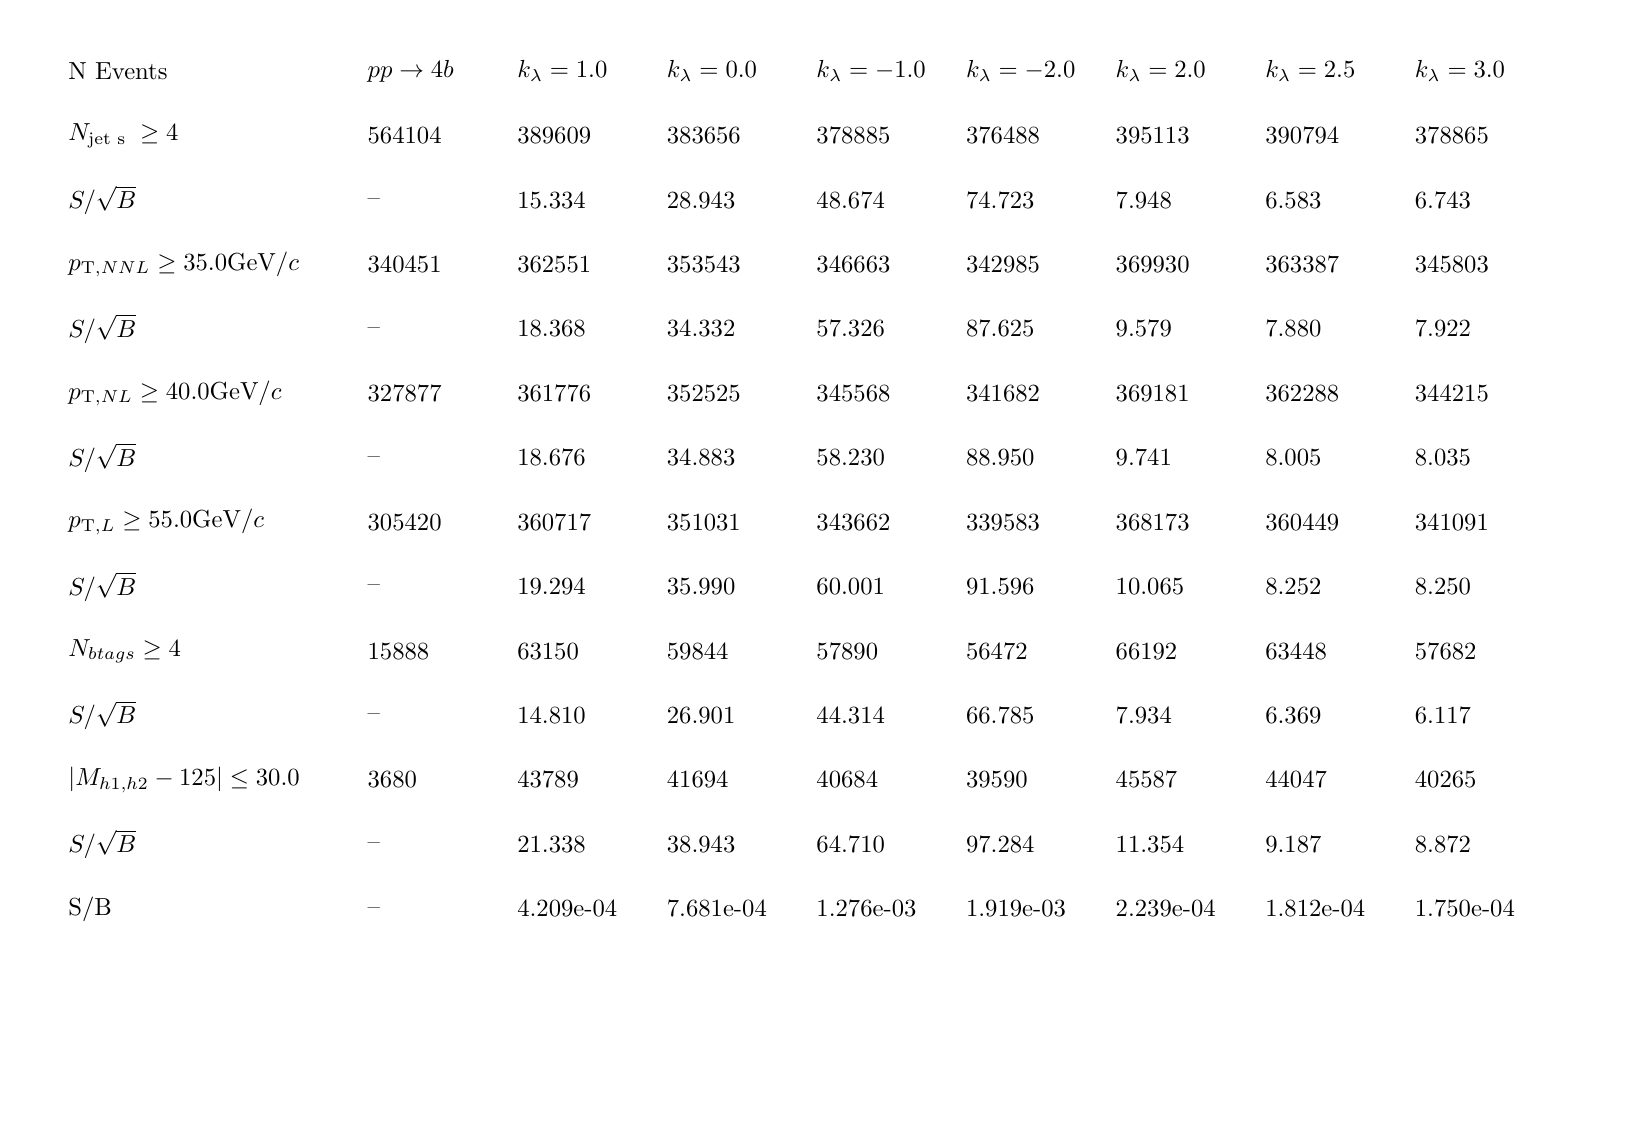
\begin{tikzpicture}
\pgfdeclareplotmark{cross} {
\pgfpathmoveto{\pgfpoint{-0.3\pgfplotmarksize}{\pgfplotmarksize}}
\pgfpathlineto{\pgfpoint{+0.3\pgfplotmarksize}{\pgfplotmarksize}}
\pgfpathlineto{\pgfpoint{+0.3\pgfplotmarksize}{0.3\pgfplotmarksize}}
\pgfpathlineto{\pgfpoint{+1\pgfplotmarksize}{0.3\pgfplotmarksize}}
\pgfpathlineto{\pgfpoint{+1\pgfplotmarksize}{-0.3\pgfplotmarksize}}
\pgfpathlineto{\pgfpoint{+0.3\pgfplotmarksize}{-0.3\pgfplotmarksize}}
\pgfpathlineto{\pgfpoint{+0.3\pgfplotmarksize}{-1.\pgfplotmarksize}}
\pgfpathlineto{\pgfpoint{-0.3\pgfplotmarksize}{-1.\pgfplotmarksize}}
\pgfpathlineto{\pgfpoint{-0.3\pgfplotmarksize}{-0.3\pgfplotmarksize}}
\pgfpathlineto{\pgfpoint{-1.\pgfplotmarksize}{-0.3\pgfplotmarksize}}
\pgfpathlineto{\pgfpoint{-1.\pgfplotmarksize}{0.3\pgfplotmarksize}}
\pgfpathlineto{\pgfpoint{-0.3\pgfplotmarksize}{0.3\pgfplotmarksize}}
\pgfpathclose
\pgfusepathqstroke
}
\pgfdeclareplotmark{cross*} {
\pgfpathmoveto{\pgfpoint{-0.3\pgfplotmarksize}{\pgfplotmarksize}}
\pgfpathlineto{\pgfpoint{+0.3\pgfplotmarksize}{\pgfplotmarksize}}
\pgfpathlineto{\pgfpoint{+0.3\pgfplotmarksize}{0.3\pgfplotmarksize}}
\pgfpathlineto{\pgfpoint{+1\pgfplotmarksize}{0.3\pgfplotmarksize}}
\pgfpathlineto{\pgfpoint{+1\pgfplotmarksize}{-0.3\pgfplotmarksize}}
\pgfpathlineto{\pgfpoint{+0.3\pgfplotmarksize}{-0.3\pgfplotmarksize}}
\pgfpathlineto{\pgfpoint{+0.3\pgfplotmarksize}{-1.\pgfplotmarksize}}
\pgfpathlineto{\pgfpoint{-0.3\pgfplotmarksize}{-1.\pgfplotmarksize}}
\pgfpathlineto{\pgfpoint{-0.3\pgfplotmarksize}{-0.3\pgfplotmarksize}}
\pgfpathlineto{\pgfpoint{-1.\pgfplotmarksize}{-0.3\pgfplotmarksize}}
\pgfpathlineto{\pgfpoint{-1.\pgfplotmarksize}{0.3\pgfplotmarksize}}
\pgfpathlineto{\pgfpoint{-0.3\pgfplotmarksize}{0.3\pgfplotmarksize}}
\pgfpathclose
\pgfusepathqfillstroke
}
\pgfdeclareplotmark{newstar} {
\pgfpathmoveto{\pgfqpoint{0pt}{\pgfplotmarksize}}
\pgfpathlineto{\pgfqpointpolar{44}{0.5\pgfplotmarksize}}
\pgfpathlineto{\pgfqpointpolar{18}{\pgfplotmarksize}}
\pgfpathlineto{\pgfqpointpolar{-20}{0.5\pgfplotmarksize}}
\pgfpathlineto{\pgfqpointpolar{-54}{\pgfplotmarksize}}
\pgfpathlineto{\pgfqpointpolar{-90}{0.5\pgfplotmarksize}}
\pgfpathlineto{\pgfqpointpolar{234}{\pgfplotmarksize}}
\pgfpathlineto{\pgfqpointpolar{198}{0.5\pgfplotmarksize}}
\pgfpathlineto{\pgfqpointpolar{162}{\pgfplotmarksize}}
\pgfpathlineto{\pgfqpointpolar{134}{0.5\pgfplotmarksize}}
\pgfpathclose
\pgfusepathqstroke
}
\pgfdeclareplotmark{newstar*} {
\pgfpathmoveto{\pgfqpoint{0pt}{\pgfplotmarksize}}
\pgfpathlineto{\pgfqpointpolar{44}{0.5\pgfplotmarksize}}
\pgfpathlineto{\pgfqpointpolar{18}{\pgfplotmarksize}}
\pgfpathlineto{\pgfqpointpolar{-20}{0.5\pgfplotmarksize}}
\pgfpathlineto{\pgfqpointpolar{-54}{\pgfplotmarksize}}
\pgfpathlineto{\pgfqpointpolar{-90}{0.5\pgfplotmarksize}}
\pgfpathlineto{\pgfqpointpolar{234}{\pgfplotmarksize}}
\pgfpathlineto{\pgfqpointpolar{198}{0.5\pgfplotmarksize}}
\pgfpathlineto{\pgfqpointpolar{162}{\pgfplotmarksize}}
\pgfpathlineto{\pgfqpointpolar{134}{0.5\pgfplotmarksize}}
\pgfpathclose
\pgfusepathqfillstroke
}
\definecolor{c}{rgb}{1,1,1};
\draw [color=c, fill=c] (0,0) rectangle (20,13.639);
\definecolor{c}{rgb}{0,0,0};
\draw [anchor= west] (0.4,13.0934) node[scale=0.890934, color=c, rotate=0]{N Events};
\draw [anchor= west] (4.2,13.0934) node[scale=0.890934, color=c, rotate=0]{$pp \rightarrow 4b$};
\draw [anchor= west] (6.1,13.0934) node[scale=0.890934, color=c, rotate=0]{$k_{\lambda} = 1.0$};
\draw [anchor= west] (8,13.0934) node[scale=0.890934, color=c, rotate=0]{$k_{\lambda} = 0.0$};
\draw [anchor= west] (9.9,13.0934) node[scale=0.890934, color=c, rotate=0]{$k_{\lambda} = -1.0$};
\draw [anchor= west] (11.8,13.0934) node[scale=0.890934, color=c, rotate=0]{$k_{\lambda} = -2.0$};
\draw [anchor= west] (13.7,13.0934) node[scale=0.890934, color=c, rotate=0]{$k_{\lambda} = 2.0$};
\draw [anchor= west] (15.6,13.0934) node[scale=0.890934, color=c, rotate=0]{$k_{\lambda} = 2.5$};
\draw [anchor= west] (17.5,13.0934) node[scale=0.890934, color=c, rotate=0]{$k_{\lambda} = 3.0$};
\draw [anchor= west] (0.4,12.2751) node[scale=0.890934, color=c, rotate=0]{$N_{\text{\text{jet~}s~}} \geq 4$};
\draw [anchor= west] (4.2,12.2751) node[scale=0.890934, color=c, rotate=0]{564104};
\draw [anchor= west] (6.1,12.2751) node[scale=0.890934, color=c, rotate=0]{389609};
\draw [anchor= west] (8,12.2751) node[scale=0.890934, color=c, rotate=0]{383656};
\draw [anchor= west] (9.9,12.2751) node[scale=0.890934, color=c, rotate=0]{378885};
\draw [anchor= west] (11.8,12.2751) node[scale=0.890934, color=c, rotate=0]{376488};
\draw [anchor= west] (13.7,12.2751) node[scale=0.890934, color=c, rotate=0]{395113};
\draw [anchor= west] (15.6,12.2751) node[scale=0.890934, color=c, rotate=0]{390794};
\draw [anchor= west] (17.5,12.2751) node[scale=0.890934, color=c, rotate=0]{378865};
\draw [anchor= west] (0.4,11.4567) node[scale=0.890934, color=c, rotate=0]{$S/\sqrt{B}$};
\draw [anchor= west] (4.2,11.4567) node[scale=0.890934, color=c, rotate=0]{--};
\draw [anchor= west] (6.1,11.4567) node[scale=0.890934, color=c, rotate=0]{15.334};
\draw [anchor= west] (8,11.4567) node[scale=0.890934, color=c, rotate=0]{28.943};
\draw [anchor= west] (9.9,11.4567) node[scale=0.890934, color=c, rotate=0]{48.674};
\draw [anchor= west] (11.8,11.4567) node[scale=0.890934, color=c, rotate=0]{74.723};
\draw [anchor= west] (13.7,11.4567) node[scale=0.890934, color=c, rotate=0]{7.948};
\draw [anchor= west] (15.6,11.4567) node[scale=0.890934, color=c, rotate=0]{6.583};
\draw [anchor= west] (17.5,11.4567) node[scale=0.890934, color=c, rotate=0]{6.743};
\draw [anchor= west] (0.4,10.6384) node[scale=0.890934, color=c, rotate=0]{$p_{\text{T}, NNL} \geq 35.0 \text{GeV}/c$};
\draw [anchor= west] (4.2,10.6384) node[scale=0.890934, color=c, rotate=0]{340451};
\draw [anchor= west] (6.1,10.6384) node[scale=0.890934, color=c, rotate=0]{362551};
\draw [anchor= west] (8,10.6384) node[scale=0.890934, color=c, rotate=0]{353543};
\draw [anchor= west] (9.9,10.6384) node[scale=0.890934, color=c, rotate=0]{346663};
\draw [anchor= west] (11.8,10.6384) node[scale=0.890934, color=c, rotate=0]{342985};
\draw [anchor= west] (13.7,10.6384) node[scale=0.890934, color=c, rotate=0]{369930};
\draw [anchor= west] (15.6,10.6384) node[scale=0.890934, color=c, rotate=0]{363387};
\draw [anchor= west] (17.5,10.6384) node[scale=0.890934, color=c, rotate=0]{345803};
\draw [anchor= west] (0.4,9.82006) node[scale=0.890934, color=c, rotate=0]{$S/\sqrt{B}$};
\draw [anchor= west] (4.2,9.82006) node[scale=0.890934, color=c, rotate=0]{--};
\draw [anchor= west] (6.1,9.82006) node[scale=0.890934, color=c, rotate=0]{18.368};
\draw [anchor= west] (8,9.82006) node[scale=0.890934, color=c, rotate=0]{34.332};
\draw [anchor= west] (9.9,9.82006) node[scale=0.890934, color=c, rotate=0]{57.326};
\draw [anchor= west] (11.8,9.82006) node[scale=0.890934, color=c, rotate=0]{87.625};
\draw [anchor= west] (13.7,9.82006) node[scale=0.890934, color=c, rotate=0]{9.579};
\draw [anchor= west] (15.6,9.82006) node[scale=0.890934, color=c, rotate=0]{7.880};
\draw [anchor= west] (17.5,9.82006) node[scale=0.890934, color=c, rotate=0]{7.922};
\draw [anchor= west] (0.4,9.00172) node[scale=0.890934, color=c, rotate=0]{$p_{\text{T}, NL} \geq 40.0 \text{GeV}/c$};
\draw [anchor= west] (4.2,9.00172) node[scale=0.890934, color=c, rotate=0]{327877};
\draw [anchor= west] (6.1,9.00172) node[scale=0.890934, color=c, rotate=0]{361776};
\draw [anchor= west] (8,9.00172) node[scale=0.890934, color=c, rotate=0]{352525};
\draw [anchor= west] (9.9,9.00172) node[scale=0.890934, color=c, rotate=0]{345568};
\draw [anchor= west] (11.8,9.00172) node[scale=0.890934, color=c, rotate=0]{341682};
\draw [anchor= west] (13.7,9.00172) node[scale=0.890934, color=c, rotate=0]{369181};
\draw [anchor= west] (15.6,9.00172) node[scale=0.890934, color=c, rotate=0]{362288};
\draw [anchor= west] (17.5,9.00172) node[scale=0.890934, color=c, rotate=0]{344215};
\draw [anchor= west] (0.4,8.18338) node[scale=0.890934, color=c, rotate=0]{$S/\sqrt{B}$};
\draw [anchor= west] (4.2,8.18338) node[scale=0.890934, color=c, rotate=0]{--};
\draw [anchor= west] (6.1,8.18338) node[scale=0.890934, color=c, rotate=0]{18.676};
\draw [anchor= west] (8,8.18338) node[scale=0.890934, color=c, rotate=0]{34.883};
\draw [anchor= west] (9.9,8.18338) node[scale=0.890934, color=c, rotate=0]{58.230};
\draw [anchor= west] (11.8,8.18338) node[scale=0.890934, color=c, rotate=0]{88.950};
\draw [anchor= west] (13.7,8.18338) node[scale=0.890934, color=c, rotate=0]{9.741};
\draw [anchor= west] (15.6,8.18338) node[scale=0.890934, color=c, rotate=0]{8.005};
\draw [anchor= west] (17.5,8.18338) node[scale=0.890934, color=c, rotate=0]{8.035};
\draw [anchor= west] (0.4,7.36504) node[scale=0.890934, color=c, rotate=0]{$p_{\text{T}, L} \geq 55.0 \text{GeV}/c$};
\draw [anchor= west] (4.2,7.36504) node[scale=0.890934, color=c, rotate=0]{305420};
\draw [anchor= west] (6.1,7.36504) node[scale=0.890934, color=c, rotate=0]{360717};
\draw [anchor= west] (8,7.36504) node[scale=0.890934, color=c, rotate=0]{351031};
\draw [anchor= west] (9.9,7.36504) node[scale=0.890934, color=c, rotate=0]{343662};
\draw [anchor= west] (11.8,7.36504) node[scale=0.890934, color=c, rotate=0]{339583};
\draw [anchor= west] (13.7,7.36504) node[scale=0.890934, color=c, rotate=0]{368173};
\draw [anchor= west] (15.6,7.36504) node[scale=0.890934, color=c, rotate=0]{360449};
\draw [anchor= west] (17.5,7.36504) node[scale=0.890934, color=c, rotate=0]{341091};
\draw [anchor= west] (0.4,6.5467) node[scale=0.890934, color=c, rotate=0]{$S/\sqrt{B}$};
\draw [anchor= west] (4.2,6.5467) node[scale=0.890934, color=c, rotate=0]{--};
\draw [anchor= west] (6.1,6.5467) node[scale=0.890934, color=c, rotate=0]{19.294};
\draw [anchor= west] (8,6.5467) node[scale=0.890934, color=c, rotate=0]{35.990};
\draw [anchor= west] (9.9,6.5467) node[scale=0.890934, color=c, rotate=0]{60.001};
\draw [anchor= west] (11.8,6.5467) node[scale=0.890934, color=c, rotate=0]{91.596};
\draw [anchor= west] (13.7,6.5467) node[scale=0.890934, color=c, rotate=0]{10.065};
\draw [anchor= west] (15.6,6.5467) node[scale=0.890934, color=c, rotate=0]{8.252};
\draw [anchor= west] (17.5,6.5467) node[scale=0.890934, color=c, rotate=0]{8.250};
\draw [anchor= west] (0.4,5.72837) node[scale=0.890934, color=c, rotate=0]{$N_{btags} \geq 4$};
\draw [anchor= west] (4.2,5.72837) node[scale=0.890934, color=c, rotate=0]{15888};
\draw [anchor= west] (6.1,5.72837) node[scale=0.890934, color=c, rotate=0]{63150};
\draw [anchor= west] (8,5.72837) node[scale=0.890934, color=c, rotate=0]{59844};
\draw [anchor= west] (9.9,5.72837) node[scale=0.890934, color=c, rotate=0]{57890};
\draw [anchor= west] (11.8,5.72837) node[scale=0.890934, color=c, rotate=0]{56472};
\draw [anchor= west] (13.7,5.72837) node[scale=0.890934, color=c, rotate=0]{66192};
\draw [anchor= west] (15.6,5.72837) node[scale=0.890934, color=c, rotate=0]{63448};
\draw [anchor= west] (17.5,5.72837) node[scale=0.890934, color=c, rotate=0]{57682};
\draw [anchor= west] (0.4,4.91003) node[scale=0.890934, color=c, rotate=0]{$S/\sqrt{B}$};
\draw [anchor= west] (4.2,4.91003) node[scale=0.890934, color=c, rotate=0]{--};
\draw [anchor= west] (6.1,4.91003) node[scale=0.890934, color=c, rotate=0]{14.810};
\draw [anchor= west] (8,4.91003) node[scale=0.890934, color=c, rotate=0]{26.901};
\draw [anchor= west] (9.9,4.91003) node[scale=0.890934, color=c, rotate=0]{44.314};
\draw [anchor= west] (11.8,4.91003) node[scale=0.890934, color=c, rotate=0]{66.785};
\draw [anchor= west] (13.7,4.91003) node[scale=0.890934, color=c, rotate=0]{7.934};
\draw [anchor= west] (15.6,4.91003) node[scale=0.890934, color=c, rotate=0]{6.369};
\draw [anchor= west] (17.5,4.91003) node[scale=0.890934, color=c, rotate=0]{6.117};
\draw [anchor= west] (0.4,4.09169) node[scale=0.890934, color=c, rotate=0]{$|M_{h1,h2} - 125|  \leq 30.0$};
\draw [anchor= west] (4.2,4.09169) node[scale=0.890934, color=c, rotate=0]{3680};
\draw [anchor= west] (6.1,4.09169) node[scale=0.890934, color=c, rotate=0]{43789};
\draw [anchor= west] (8,4.09169) node[scale=0.890934, color=c, rotate=0]{41694};
\draw [anchor= west] (9.9,4.09169) node[scale=0.890934, color=c, rotate=0]{40684};
\draw [anchor= west] (11.8,4.09169) node[scale=0.890934, color=c, rotate=0]{39590};
\draw [anchor= west] (13.7,4.09169) node[scale=0.890934, color=c, rotate=0]{45587};
\draw [anchor= west] (15.6,4.09169) node[scale=0.890934, color=c, rotate=0]{44047};
\draw [anchor= west] (17.5,4.09169) node[scale=0.890934, color=c, rotate=0]{40265};
\draw [anchor= west] (0.4,3.27335) node[scale=0.890934, color=c, rotate=0]{$S/\sqrt{B}$};
\draw [anchor= west] (4.2,3.27335) node[scale=0.890934, color=c, rotate=0]{--};
\draw [anchor= west] (6.1,3.27335) node[scale=0.890934, color=c, rotate=0]{21.338};
\draw [anchor= west] (8,3.27335) node[scale=0.890934, color=c, rotate=0]{38.943};
\draw [anchor= west] (9.9,3.27335) node[scale=0.890934, color=c, rotate=0]{64.710};
\draw [anchor= west] (11.8,3.27335) node[scale=0.890934, color=c, rotate=0]{97.284};
\draw [anchor= west] (13.7,3.27335) node[scale=0.890934, color=c, rotate=0]{11.354};
\draw [anchor= west] (15.6,3.27335) node[scale=0.890934, color=c, rotate=0]{9.187};
\draw [anchor= west] (17.5,3.27335) node[scale=0.890934, color=c, rotate=0]{8.872};
\draw [anchor= west] (0.4,2.45501) node[scale=0.890934, color=c, rotate=0]{S/B};
\draw [anchor= west] (4.2,2.45501) node[scale=0.890934, color=c, rotate=0]{--};
\draw [anchor= west] (6.1,2.45501) node[scale=0.890934, color=c, rotate=0]{4.209e-04};
\draw [anchor= west] (8,2.45501) node[scale=0.890934, color=c, rotate=0]{7.681e-04};
\draw [anchor= west] (9.9,2.45501) node[scale=0.890934, color=c, rotate=0]{1.276e-03};
\draw [anchor= west] (11.8,2.45501) node[scale=0.890934, color=c, rotate=0]{1.919e-03};
\draw [anchor= west] (13.7,2.45501) node[scale=0.890934, color=c, rotate=0]{2.239e-04};
\draw [anchor= west] (15.6,2.45501) node[scale=0.890934, color=c, rotate=0]{1.812e-04};
\draw [anchor= west] (17.5,2.45501) node[scale=0.890934, color=c, rotate=0]{1.750e-04};
\end{tikzpicture}
% end document
\end{document}
